\documentclass[wide,a4paper,titlepage,12pt] {article}
\usepackage{polski}
\usepackage[utf8]{inputenc}
\usepackage{listings}
\usepackage{slashbox}
\usepackage[table]{xcolor}
\usepackage{graphicx,pdflscape}
\usepackage{placeins}

\title{Układy cyfrowe i systemy wbudowane}
\author{Tymon Tobolski (181037)\\ Jacek Wieczorek (181043)}

% Title page layout (fold)
\makeatletter
\renewcommand{\maketitle}{
\begin{titlepage}
  \begin{center}
    \vspace*{3cm}
    \LARGE \@title \par
    \vspace{2cm}
    \textit{\small Autor:}\par
    \normalsize \@author\par \normalsize
    \vspace{3cm}
    \textit{\small Prowadzący:}\par
    Dr inż. Jarosław Sugier \par
    \vspace{2cm}
    Wydział Elektroniki\\ III rok\\ Pn 14.15 - 16.00\par
    \vspace{4cm}
    \small \@date
  \end{center}
\end{titlepage}
}
\makeatother

\begin{document}
\maketitle
  \section{Zadanie nr 1}
  Celem zadania było zamodelowanie układu detektora sekwencji 1 1 0 0 0 przy pomocy automatu Mealy'ego, przetestowanie jego działania w symulatorze, a następnie uruchomienie go na płycie $ZL-9572$. Układ miał za zadanie zapalić diodę LED w momencie wykrycia sekwencji.

  \begin{figure}[htbp]
    \begin{center}
      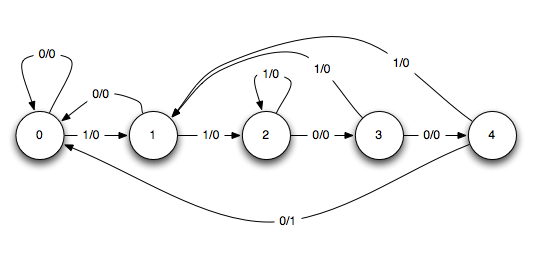
\includegraphics[scale=0.7]{mealy-graf.png}
      \caption{Graf automatu Mealy'ego}
     \end{center}
  \end{figure}


  W celu wyznaczenia odpowiednich kombinacji syngałów dla wejść przerzutników zostosowana została metoda siatek Karnaugh.


  \begin{center}
    \begin{tabular}{|c|c|c|c||c|c|c|c|}
      \hline
      $Q_{2}$ & $Q_{1}$ & $Q_{0}$ & $X$ & $Q_{2}$ & $Q_{1}$ & $Q_{0}$ & $Y$ \\
      \hline
      0 & 0 & 0 & 0 & 0 & 0 & 0 & 0 \\
      0 & 0 & 0 & 1 & 0 & 0 & 1 & 0 \\
      0 & 0 & 1 & 0 & 0 & 0 & 0 & 0 \\
      0 & 0 & 1 & 1 & 0 & 1 & 0 & 0 \\
      0 & 1 & 0 & 0 & 0 & 1 & 1 & 0 \\
      0 & 1 & 0 & 1 & 0 & 1 & 0 & 0 \\
      0 & 1 & 1 & 0 & 1 & 0 & 0 & 0 \\
      0 & 1 & 1 & 1 & 0 & 0 & 1 & 0 \\
      1 & 0 & 0 & 0 & 0 & 0 & 0 & 1 \\
      1 & 0 & 0 & 1 & 0 & 0 & 1 & 0 \\
      \hline
    \end{tabular}
  \end{center}

  \begin{center}
    \begin{tabular}{|c|c|c|c|c|}
    \hline
    \backslashbox{$Q_{0}$$X$}{$Q_{2}$$Q_{1}$} & 00 & 01 & 11 & 10 \\ \hline
    00 & 0 & 0 & * & 0 \\ \hline
    01 & 0 & 0 & * & 0 \\ \hline
    11 & 0 & 0 & * & * \\ \hline
    10 & 0 & \cellcolor[gray]{0.8}1 & \cellcolor[gray]{0.8}* & * \\ \hline
    \end{tabular}
    \\ $Q_{2}'$ = $Q_{1} Q_{0} X$
  \end{center}

  \begin{center}
    \begin{tabular}{|c|c|c|c|c|}
    \hline
    \backslashbox{$Q_{0}$$X$}{$Q_{2}$$Q_{1}$} & 00 & 01 & 11 & 10 \\ \hline
    00 & 0 & \cellcolor[gray]{0.8}1 & \cellcolor[gray]{0.8}* & 0 \\ \hline
    01 & 0 & \cellcolor[gray]{0.8}1 & \cellcolor[gray]{0.8}* & 0 \\ \hline
    11 & \cellcolor[gray]{0.8}1 & 0 & * & \cellcolor[gray]{0.8}* \\ \hline
    10 & 0 & 0 & * & * \\ \hline
    \end{tabular}
    \\ $Q_{1}'$ = $Q_{1} \bar{Q_{0}} + \bar{Q_{1}} Q_{0} X $
  \end{center}

  \begin{center}
    \begin{tabular}{|c|c|c|c|c|}
    \hline
    \backslashbox{$Q_{0}$$X$}{$Q_{2}$$Q_{1}$} & 00 & 01 & 11 & 10 \\ \hline
    00 & 0 & \cellcolor[gray]{0.8}1 & \cellcolor[gray]{0.8}* & 0 \\ \hline
    01 & \cellcolor[gray]{0.8}1 & 0 & * & 0 \\ \hline
    11 & 0 & \cellcolor[gray]{0.8}1 & \cellcolor[gray]{0.8}* & * \\ \hline
    10 & 0 & \cellcolor[gray]{0.8}1 & \cellcolor[gray]{0.8}* & * \\ \hline
    \end{tabular}
    \\ $Q_{1}'$ = $Q_{1} Q_{0} + Q_{1} \bar{Q_{0}} \bar{X} + \bar{Q_{2}} \bar{Q_{1}} \bar{Q_{0}} X $
  \end{center}

  \begin{center}
    $Y$ = $Q_{2} \bar{Q_{1}} \bar{Q_{0}} \bar{X} $
  \end{center}


  \begin{figure}[htbp]
    \begin{center}
      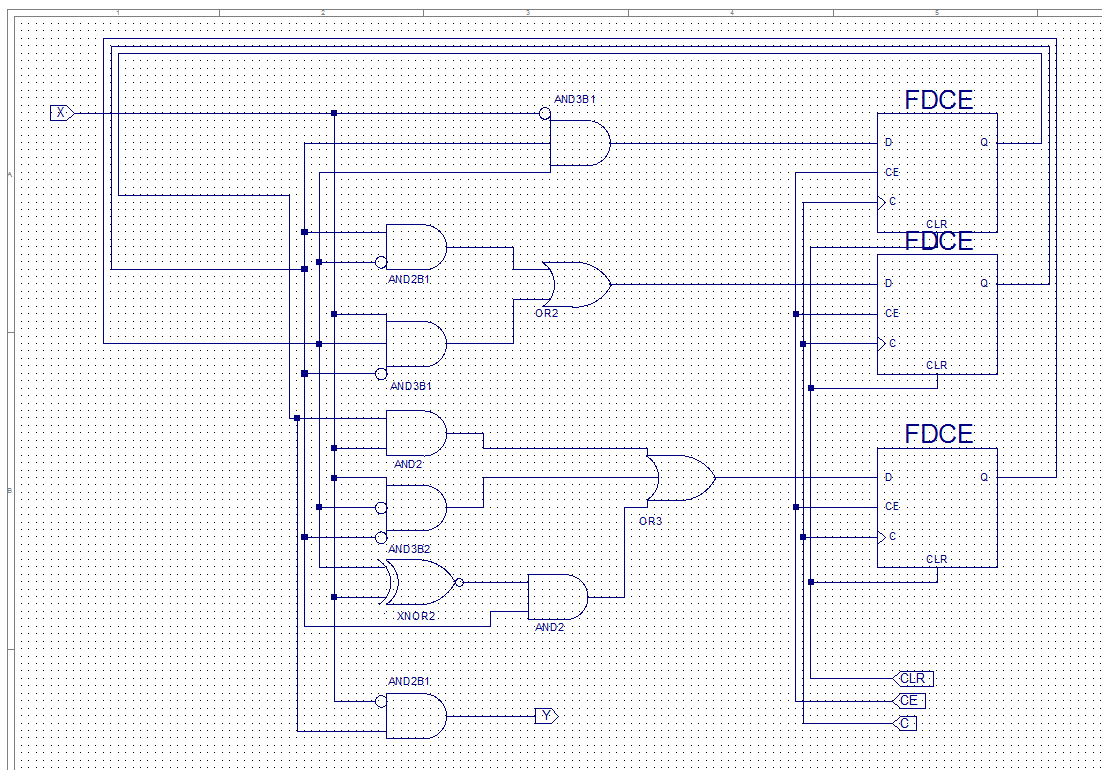
\includegraphics[scale=0.4]{mealy-sch.png}
      \caption{Schemat układu}
     \end{center}
  \end{figure}

  Następnym etapem ćwiczenia było napisanie testów oraz odpowiednie zmoodyfikownanie pliku \textit{ZL-9572.ucf} pozwalające na zasymulowanie układu.



  \newpage
  \paragraph{}
  Testy napisane w języku \textit{VHDL}
  \lstinputlisting[language=Vhdl]{code1.txt}

  Kolejnym etapem zadania było zamodelowanie działania schematu za pomocą programu ModelSim oraz zaprogramowanie urządzenia za pomocą złącza \textit{JTAG}.

  \begin{figure}[htbp]
    \begin{center}
      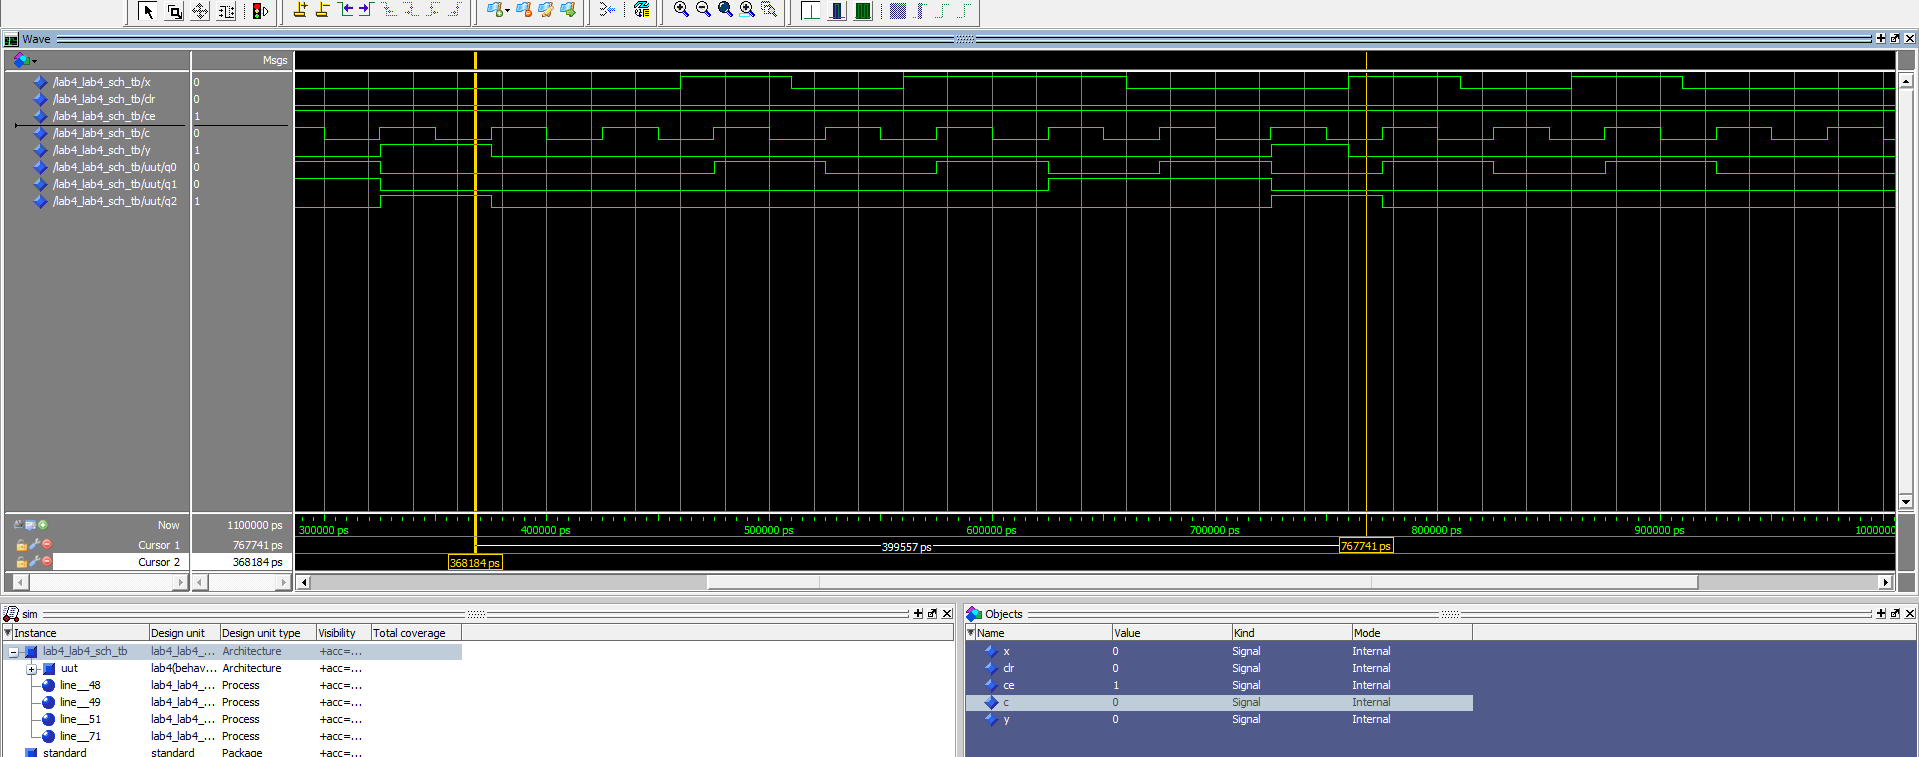
\includegraphics[scale=0.3]{mealy-sim.png}
      \caption{Przebieg symulacji}
     \end{center}
  \end{figure}

  \section{Zadanie nr 2}
  Drugim zadaniem było przerobienie automatu z zadania pierwszego na automat Moore'a.

    \begin{figure}[htbp]
    \begin{center}
      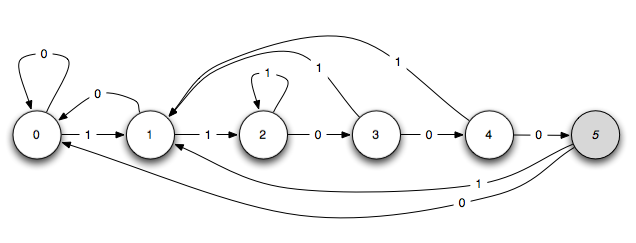
\includegraphics[scale=0.7]{moore-graf.png}
      \caption{Graf automatu Moore'a}
     \end{center}
  \end{figure}

  W celu wyznaczenia odpowiednich kombinacji syngałów dla wejść przerzutników ponownie zostosowana została metoda siatek Karnaugh.

\begin{center}
\begin{tabular}{|c|c|c|c||c|c|c|}
  \hline
  $Q_{2}$ & $Q_{1}$ & $Q_{0}$ & $X$ & $Q_{2}$ & $Q_{1}$ & $Q_{0}$ \\
  \hline
  0 & 0 & 0 & 0 & 0 & 0 & 0 \\
  0 & 0 & 0 & 1 & 0 & 0 & 1 \\
  0 & 0 & 1 & 0 & 0 & 0 & 0 \\
  0 & 0 & 1 & 1 & 0 & 1 & 0 \\
  0 & 1 & 0 & 0 & 0 & 1 & 1 \\
  0 & 1 & 0 & 1 & 0 & 1 & 0 \\
  0 & 1 & 1 & 0 & 1 & 0 & 0 \\
  0 & 1 & 1 & 1 & 0 & 0 & 1 \\
  1 & 0 & 0 & 0 & 1 & 0 & 1 \\
  1 & 0 & 0 & 1 & 0 & 0 & 1 \\
  1 & 0 & 1 & 0 & 0 & 0 & 0 \\
  1 & 0 & 1 & 1 & 0 & 0 & 1 \\
  \hline
\end{tabular}
\end{center}

  \begin{center}
    \begin{tabular}{|c|c|c|c|c|}
    \hline
    \backslashbox{$Q_{0}$$X$}{$Q_{2}$$Q_{1}$} & 00 & 01 & 11 & 10 \\ \hline
    00 & 0 & 0 &\cellcolor[gray]{0.8}* & \cellcolor[gray]{0.8}1 \\ \hline
    01 & 0 & 0 & * & 0 \\ \hline
    11 & 0 & 0 & * & 0 \\ \hline
    10 & 0 &\cellcolor[gray]{0.8}1 & \cellcolor[gray]{0.8}* & 0 \\ \hline
    \end{tabular}
    \\ $Q_{2}'$ = $Q_{2} \bar{Q_{0}}\bar{X} +  Q_{1}Q_{0}\bar{X}$
  \end{center}

  \begin{center}
    \begin{tabular}{|c|c|c|c|c|}
    \hline
    \backslashbox{$Q_{0}$$X$}{$Q_{2}$$Q_{1}$} & 00 & 01 & 11 & 10 \\ \hline
    00 & 0 & \cellcolor[gray]{0.8}1 & \cellcolor[gray]{0.8}* & 0 \\ \hline
    01 & 0 & \cellcolor[gray]{0.8}1 & \cellcolor[gray]{0.8}* & 0 \\ \hline
    11 & \cellcolor[gray]{0.8}1 & 0 & * & 0 \\ \hline
    10 & 0 & 0 & * & 0 \\ \hline
    \end{tabular}
    \\ $Q_{2}'$ = $Q_{1} \bar{Q_{0}} +  \bar{Q_{2}} \bar{Q_{1}} Q_{0} X$
  \end{center}


\begin{center}
  \begin{tabular}{|c|c|c|c|c|}
  \hline
  \backslashbox{$Q_{0}$$X$}{$Q_{2}$$Q_{1}$} & 00 & 01 & 11 & 10 \\ \hline
  00 & 0 & \cellcolor[gray]{0.8}1 & \cellcolor[gray]{0.8}* & \cellcolor[gray]{0.8}1 \\ \hline
  01 & \cellcolor[gray]{0.8} 1 & 0 &  \cellcolor[gray]{0.8}* & \cellcolor[gray]{0.8}1 \\ \hline
  11 & 0 & \cellcolor[gray]{0.8} 1 & \cellcolor[gray]{0.8}* & \cellcolor[gray]{0.8}1 \\ \hline
  10 & 0 & 0 & * & 0 \\ \hline
  \end{tabular}
  \\ $Q_{0}'$ = $Q_{1} \bar{Q_{0}} \bar{X} + \bar{Q_{1}} \bar{Q_{0}} X + \bar{Q_{1}} Q_{0} X + Q_{2} \bar{Q_{0}} + Q_{2} X$
\end{center}


  \begin{figure}[htbp]
    \begin{center}
      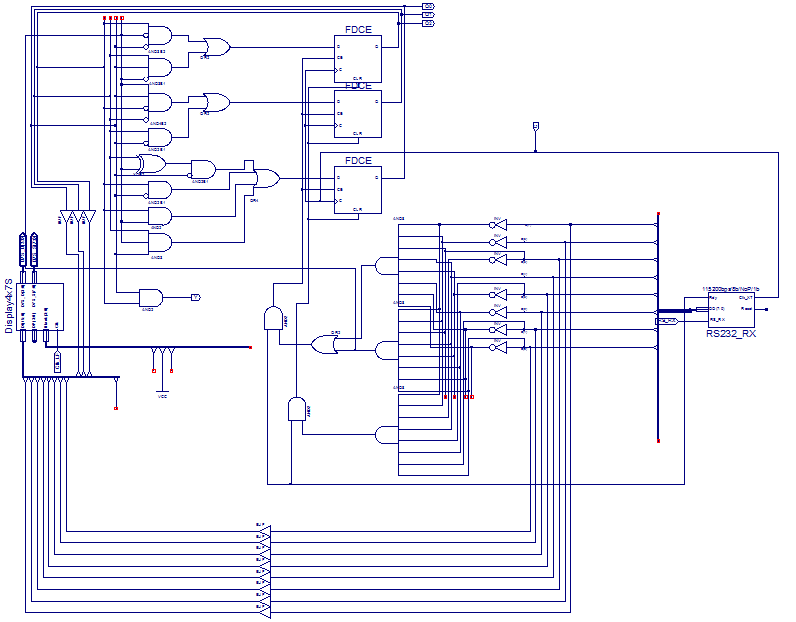
\includegraphics[scale=0.6]{moore-sch.png}
      \caption{Schemat układu}
     \end{center}
  \end{figure}

Do testowania automaty Moore'a wykorzystane zostały identyczne testy jak dla automatu z zadania pierwszego.

\paragraph{}

  \begin{figure}[htbp]
    \begin{center}
      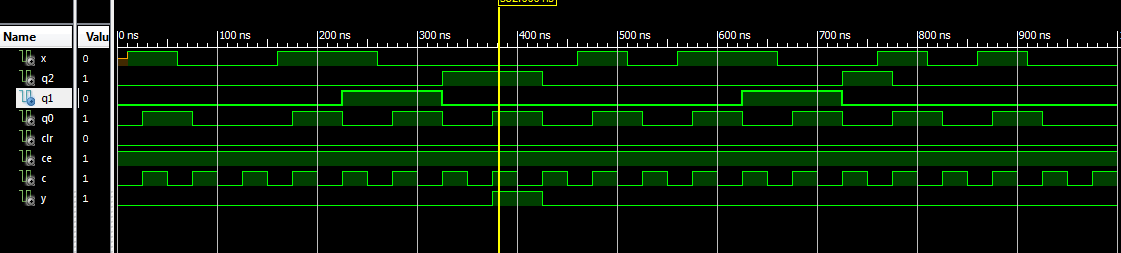
\includegraphics[scale=0.5]{moore-sim.png}
      \caption{Przebieg symulacji}
     \end{center}
  \end{figure}

Dodatkowymi zadaniami do zrealizowania było zaimplementowanie sterowania automatem z klawiatury komputera poprzez podłączenie układu za pomocą portu szeregowego. Wciśnięcie klawisza $1$ (kod 49) lub $0$ (kod 48) powodowało sprawdzenie kolejnej cyfry sekwencji przez układ. Klawisz $Esc$ (kod 27) służył do resetowania sekwencji. Wszelkie inne klawisze były ignorowane przez układ.

\paragraph{}

Kolejnym zadaniem dodatkowym było wyświetlenie kodu wysyłanego klawisza na wyświetlaczu 7-segmentowym. Ponadto na wyświetlaczu umieściliśmy również numer aktualnego stanu urządzenia.

  \newpage
  \section{Wnioski}
  Po wykonaniu testów i symulacji okazało się, iż automat Mealy'ego jest podatny na "oszustwo".

\end{document}



